\documentclass[12pt]{article}
\author{Lawrence Liu}
\usepackage{subcaption}
\usepackage{graphicx}
\usepackage{amsmath}
\usepackage{pdfpages}
\newcommand{\Laplace}{\mathscr{L}}
\setlength{\parskip}{\baselineskip}%
\setlength{\parindent}{0pt}%
\usepackage{xcolor}
\usepackage{listings}
\definecolor{backcolour}{rgb}{0.95,0.95,0.92}
\usepackage{amssymb}
\lstdefinestyle{mystyle}{
    backgroundcolor=\color{backcolour}}
\lstset{style=mystyle}

\title{ECE 231A HW 3}
\begin{document}
\maketitle
\section*{Problem 1}
\subsection*{(a)}
\begin{align*}
    \lim_{n\to\infty}[p(X_1,\cdots,X_n)]^{\frac{1}{n}}&=
        2^{\lim_{n\to\infty}\frac{1}{n}\log_2[p(X_1,\cdots,X_n)]}\\
    &=2^{\lim_{n\to\infty}\frac{1}{n}\sum_{i=1}^n\log_2[p(X_i)]}\\
    &=2^{E[\ln[p(X_i)]]}\\
    &=\boxed{2^{-H(x)}}
\end{align*}
\subsection*{(b)}
\begin{align*}
    E\left[\left(\prod_{i=1}^nf(X_i)\right)^{\frac{1}{n}}\right]&=
        \left(\left(E\left[\left(\prod_{i=1}^nf(X_i)\right)^{\frac{1}{n}}\right]\right)^{n}\right)^{\frac{1}{n}}\\
        &\leq \left(E\left[\prod_{i=1}^nf(X_i)\right]\right)^{\frac{1}{n}}\\
        &=\left(E^n[f(X_1)]\right)^{\frac{1}{n}}\\
        &=E[f(X_1)]
\end{align*}
Therefore we have that
$$
    \boxed{E\left[\left(\prod_{i=1}^nf(X_i)\right)^{\frac{1}{n}}\right]\leq E[X_i]}
    $$
\section*{Problem 2}
\subsection*{(a)}
$$H(X)=\boxed{2.246 \text{ Shannons}}$$
\subsection*{(b)}
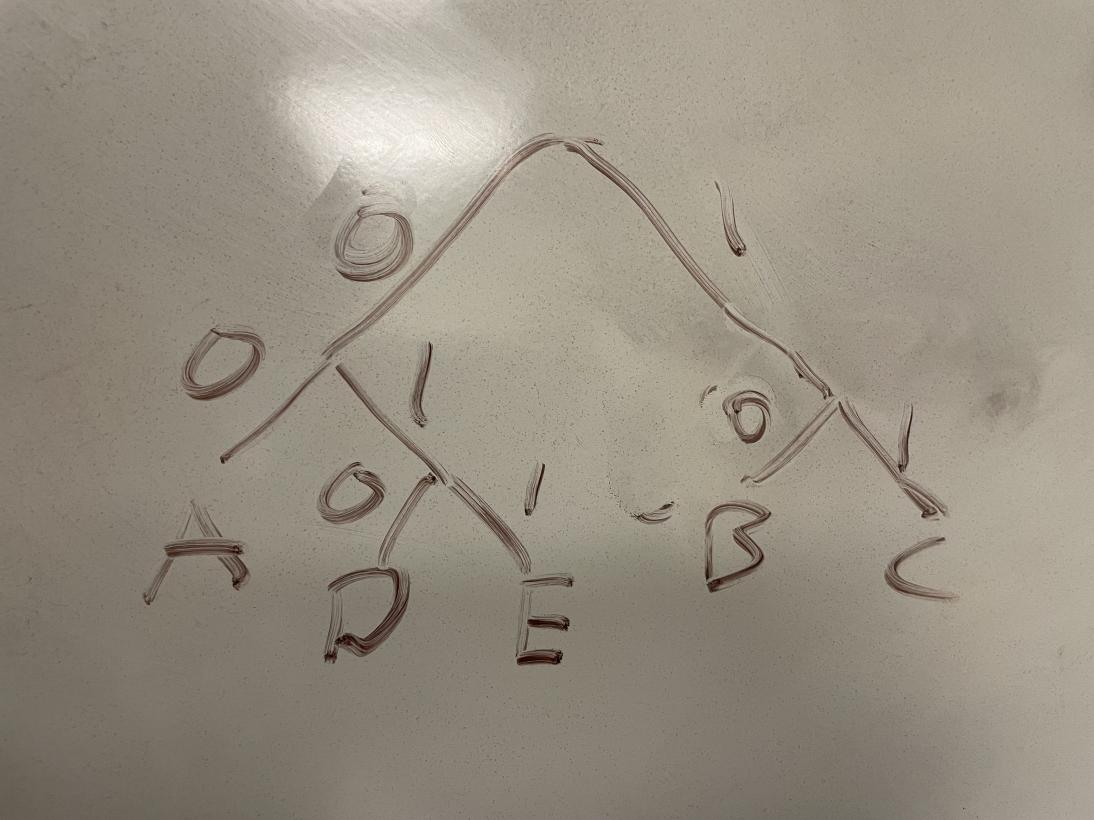
\includegraphics[scale=0.25]{fig1.jpg}\\
So we have that the average length is $\boxed{2.3}$ bits.
\subsection*{(c)}
codeword A is 001\\
codeword B is 0110\\
codeword C is 1001\\
codeword D is 1100\\
codeword E is 11110\\
Therefore the SFE codeword average length is $\boxed{3.8} bits$.
\subsection*{(d)}
We have that the CDF of $BAC$ is 
$$P(X_1=A)+P(X_1=B,X_2=A)(P(X_3=A)+P(X_3=B)+P(X_3=C))=\boxed{0.342}$$
Therefore for the SFE code, we have that 
$$\bar{F}=P(X_1=A)+P(X_1=B,X_2=A)(P(X_3=A)+P(X_3=B)+P(X_3=C))-
    \frac{1}{2}P(X_1=B,X_2=A,X_3=c)=\boxed{0.336}$$
and
$$l=-\lceil \log_2(P(X_1=B,X_2=A,X_3=c))\rceil +1=8$$
Thus we have that the SFE encoding is $\boxed{01010110}$
\section*{Problem 3}
\subsection*{(a)}
$$F(X^1)=\begin{cases}
    0.2 & \text{if }X^1=A\\
    0.5 & \text{if }X^1=B\\
    1 & \text{if }X^1=C\\
\end{cases}$$
The interval for the first symbol is $[0,0.2)$.
\subsection*{(b)}
$$F(X^1X^2)=\begin{cases}
    0.04 & \text{if }X^1X^2=AA\\
    0.1 & \text{if }X^1X^2=AB\\
    0.2 & \text{if }X^1X^2=AC\\
    0.26 & \text{if }X^1X^2=BA\\
    0.35 & \text{if }X^1X^2=BB\\
    0.5 & \text{if }X^1X^2=BC\\
    0.6 & \text{if }X^1X^2=CA\\
    0.75 & \text{if }X^1X^2=CB\\
    1 & \text{if }X^1X^2=CC
\end{cases}$$
Therefore the interval corresponding to AC is 
$[0.1,0.2)$
\subsection*{(c)}
Therefore the cdf for 
$$F(X^1X^2X^3X^4)=0.1+0.1*0.6=0.16$$
Therefore we have that 
$$\bar{F}=0.16-0.1*0.6/2=0.14$$
\end{document}